% coding:utf-8

%FOSAET, a LaTeX-Code for a electrical summary of basic electronics
%Copyright (C) 2013, Daniel Winz, Ervin Mazlagic

%This program is free software; you can redistribute it and/or
%modify it under the terms of the GNU General Public License
%as published by the Free Software Foundation; either version 2
%of the License, or (at your option) any later version.

%This program is distributed in the hope that it will be useful,
%but WITHOUT ANY WARRANTY; without even the implied warranty of
%MERCHANTABILITY or FITNESS FOR A PARTICULAR PURPOSE.  See the
%GNU General Public License for more details.
%----------------------------------------

\newpage
\section{Knotenpotentialverfahren}
\begin{enumerate}
  \item Alle realen Spannungsquellen in Stromquellen umwandeln. 
  \item Null-Potential ($N_0$) wählen (bestenfalls dort wo der Strom gesucht ist)
  \item restliche Knoten nummerieren ($N_1$, $N_2$, $N_3$ ...$N_n$)
  \item Matrix aufstellen
  \item Links alle Knoten ohne den Bezugsknoten auflisten
  \item Oben alle Spannungen von den Knoten zum Bezugsknoten eintragen
  \item Hauptdiagonale ausfüllen: \\
  Dazu sind die Leitwerte aller Widerstände, die am jeweiligen Knoten angeschlossen sind zu addieren und hinzuschreiben. 
  \item Restliche Matrix ausfüllen: \\
  Dazu sind die Leitwerte aller Widerstände, die direkt zwischen den jeweiligen Knoten liegen zu addieren und einzutragen. Das Vorzeichen ist dabei immer negativ. \\
  Liegt keine direkte Verbindung zwischen zwei Knoten, so wird 0 eingetragen
  \item In der rechten Spalte Stromquellen eintragen. \\
  Das Vorzeichen ist dabei abhängig von der Flussrichtung: \\
  \begin{itemize}
    \item[+] wenn der Strom in den Knoten fliesst
    \item[-] wenn der Strom vom Knoten weg fliesst
  \end{itemize}
\end{enumerate}

\newpage
\subsection{Beispiel}

\begin{figure}[h!]
\centering
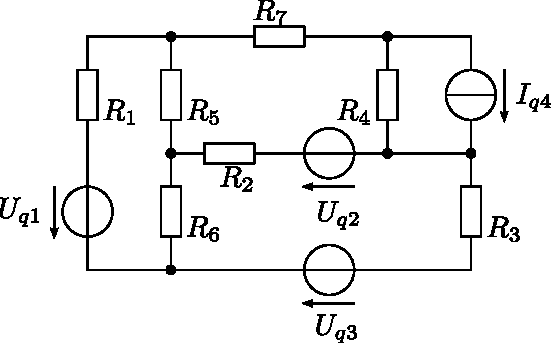
\includegraphics[scale=\schscale]{knotpot_sch.pdf}
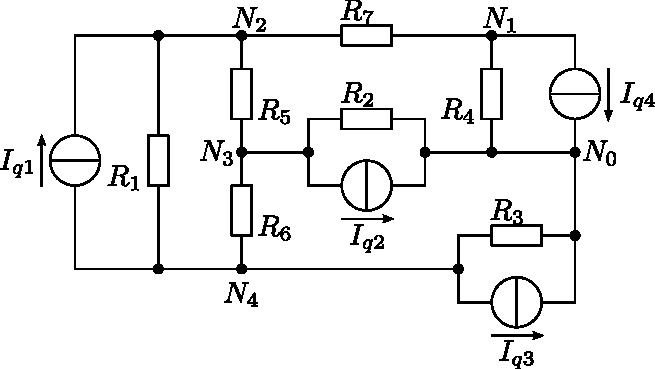
\includegraphics[scale=\schscale]{knotpot_sch_2.pdf}
\caption{Umwandlung von Strom- zu Spannungsquellen}
\label{sch:knotpot_2}
\end{figure}

\begin{table}[h!]
\footnotesize
\[ 	\begin{array}{c|cccc||c}
	N & U_{10}						& U_{20}										& U_{30} 											& U_{40} 											& I \\
	\hline &&&&& \\
	N_1	& \frac{1}{R_4} + \frac{1}{R_7}		& -\frac{1}{R_7} 								& 0 												& 0 												& -I_{q4} 			\\
	&&&&& \\
	N_2	& -\frac{1}{R_7} 					& \frac{1}{R_1} + \frac{1}{R_5} + \frac{1}{7} 	& -\frac{1}{R_5} 									& -\frac{1}{R_1} 									& I_{q1} 			\\ 
	&&&&& \\
	N_3	& 0 								& -\frac{1}{R_5} 								& \frac{1}{R_2} + \frac{1}{R_5} + \frac{1}{R_6} 	& -\frac{1}{R_6} 									& -I_{q2} 			\\ 
	&&&&& \\
	N_4 & 0 								& -\frac{1}{R_1} 								& -\frac{1}{R_6} 									& \frac{1}{R_1} + \frac{1}{R_3} + \frac{1}{R_6} 	& -I_{q2} -I_{q3} 	\\ 
	&&&&& \\
	\end{array}
\]
\normalsize
\caption{Matrix zu Abb.~\ref{sch:knotpot_2}}
\end{table}

\newpage
